% This is based on "sig-alternate.tex" V1.9 April 2009
% This file should be compiled with V2.4 of "sig-alternate.cls" April 2009
%
\documentclass{report}

\usepackage[english]{babel}
\usepackage{graphicx}
\usepackage{tabularx}
\usepackage{subfigure}
\usepackage{enumitem}
\usepackage{url}


\usepackage{color}
\definecolor{orange}{rgb}{1,0.5,0}
\definecolor{lightgray}{rgb}{.9,.9,.9}
\definecolor{java_keyword}{rgb}{0.37, 0.08, 0.25}
\definecolor{java_string}{rgb}{0.06, 0.10, 0.98}
\definecolor{java_comment}{rgb}{0.12, 0.38, 0.18}
\definecolor{java_doc}{rgb}{0.25,0.35,0.75}

% code listings

\usepackage{listings}
\lstloadlanguages{Java}
\lstset{
	language=Java,
	basicstyle=\scriptsize\ttfamily,
	backgroundcolor=\color{lightgray},
	keywordstyle=\color{java_keyword}\bfseries,
	stringstyle=\color{java_string},
	commentstyle=\color{java_comment},
	morecomment=[s][\color{java_doc}]{/**}{*/},
	tabsize=2,
	showtabs=false,
	extendedchars=true,
	showstringspaces=false,
	showspaces=false,
	breaklines=true,
	numbers=left,
	numberstyle=\tiny,
	numbersep=6pt,
	xleftmargin=3pt,
	xrightmargin=3pt,
	framexleftmargin=3pt,
	framexrightmargin=3pt,
	captionpos=b
}

% Disable single lines at the start of a paragraph (Schusterjungen)

\clubpenalty = 10000

% Disable single lines at the end of a paragraph (Hurenkinder)

\widowpenalty = 10000
\displaywidowpenalty = 10000
 
% allows for colored, easy-to-find todos

\newcommand{\todo}[1]{\textsf{\textbf{\textcolor{orange}{[[#1]]}}}}

% consistent references: use these instead of \label and \ref

\newcommand{\lsec}[1]{\label{sec:#1}}
\newcommand{\lssec}[1]{\label{ssec:#1}}
\newcommand{\lfig}[1]{\label{fig:#1}}
\newcommand{\ltab}[1]{\label{tab:#1}}
\newcommand{\rsec}[1]{Section~\ref{sec:#1}}
\newcommand{\rssec}[1]{Section~\ref{ssec:#1}}
\newcommand{\rfig}[1]{Figure~\ref{fig:#1}}
\newcommand{\rtab}[1]{Table~\ref{tab:#1}}
\newcommand{\rlst}[1]{Listing~\ref{#1}}

% General information

\title{einz\\
\normalsize{Distributed Systems -- Project Proposal}}
\subtitle{subtitle}

% Use the \alignauthor commands to handle the names
% and affiliations for an 'aesthetic maximum' of six authors.

\numberofauthors{1} %  in this sample file, there are a *total*
% of EIGHT authors. SIX appear on the 'first-page' (for formatting
% reasons) and the remaining two appear in the \additionalauthors section.
%
\author{
% You can go ahead and credit any number of authors here,
% e.g. one 'row of three' or two rows (consisting of one row of three
% and a second row of one, two or three).
%
% The command \alignauthor (no curly braces needed) should
% precede each author name, affiliation/snail-mail address and
% e-mail address. Additionally, tag each line of
% affiliation/address with \affaddr, and tag the
% e-mail address with \email.
%
% 1st. author
\alignauthor \normalsize{Clemens Bachmann, Josua Cantieni, Fabian Gessler, Christian Knieling, Eric Mink, Silvia Siegrist}\\
	\affaddr{\normalsize{ETH ID-1 13-932-488, ETH ID-2 15-919-038, ETH ID-3 15-939-341, ETH ID-4 14-923-809, ETH ID-5 15-917-057, ETH ID-6 15-935-893}}\\
	\email{\normalsize{baclemen@student.ethz.ch, two@student.ethz.ch, fgesser@student.ethz.ch, knielinc@student.ethz.ch, minker@student.ethz.ch, sisilvia@student.ethz.ch}}
}
%TODO: überprüefed eui agabe

\begin{document}

\maketitle

\begin{abstract}
This proposal should conclude the initial planning phase. This is where you choose a project, set your goals,
clarify your ideas, and find the materials you will need. 
Concisely state 
\textit{(a)}~System overview
\textit{(b)}~software and hardware you intend to use in this project,
\textit{(c)}~expected deliveries of this project.

OUR PART:
We choose to create an android application for smartphones which allows to play the game "einz" which is very similar to the popluar UNO cardgame. The goal is to be able to play this game with friends wherever you are, as long as you have a smartphone and access to the Internet.
For this purpose we will create an android application which is able to take the role of server and client at the same time. The device of one of the players is used as the server for the game which saves the state of the game and is responsible for synchronization. In this way there is no extra server needed, except for the lookup of the players in case that they are not in the same LAN.
\end{abstract}

\section{Introduction}

Introduction to the problem you are working on, why is it important and
what makes it challenging to solve, spell out the distributed systems challenges and how you plan to tackle them. 
State the technical problem you intend to solve. Indicate how it might be useful. This can be brief; it is just
an introduction to the next section.

Use this section as well for background information, particularly if your project is building on
previous work. If it is doing that, you need to refer to the work, describe it,
and say how you are extending it. What are the new ideas?

Use references such as books~\cite{hello}, papers~\cite{REST}, or specifications~\cite{RFC2616} whenever available.
Web-sites for documentation~\cite{devServices}, tutorials, etc., are a special case.
In a thesis, you would put them as footnotes.
At this stage, however, you will only have a few ``real references'',
so we put the Web-sites into the bibliography.
Cite every source you used throughout the project.\\

OUR PART:
We build a distributed game similar to then known card game "UNO". Because you might often find yourself wanting to play a game with friends - e.g. while you are waiting for the next train - but without a set of cards to play it, it would be useful to always have the cards on your body. We make this easy by implementing a similar game on the phone as a native application.\\

Obvious difficulties awaiting us include the coordination of a team consisting of six people, each with different skillsets and time available.
We intend to create an easily extensible codebase so that we can first build the base game and in a second phase add further rules without much effort. This poses difficulties on its own as we have to learn coding patterns such as using factories to make the program code more modular.\\
Technical problems will probably be the selection of one device as the server, smooth and clean communication between the clients and the server and implementing concurrency within the server.\\

For the usual difficulties in networking like message ordering and making sure the peers actually get the messages, we will rely on TCP.


\section{System Overview}

This is the core of the proposal.
It is where you spell out your technical plan and explain the project design.
Expected evaluation/demonstration issues would also be addressed in this section.
Use helpful figures such as~\rfig{example} and~\rfig{system-overview},
explain the figures in the text where you reference them. 


\begin{figure}[h]
	\centering
    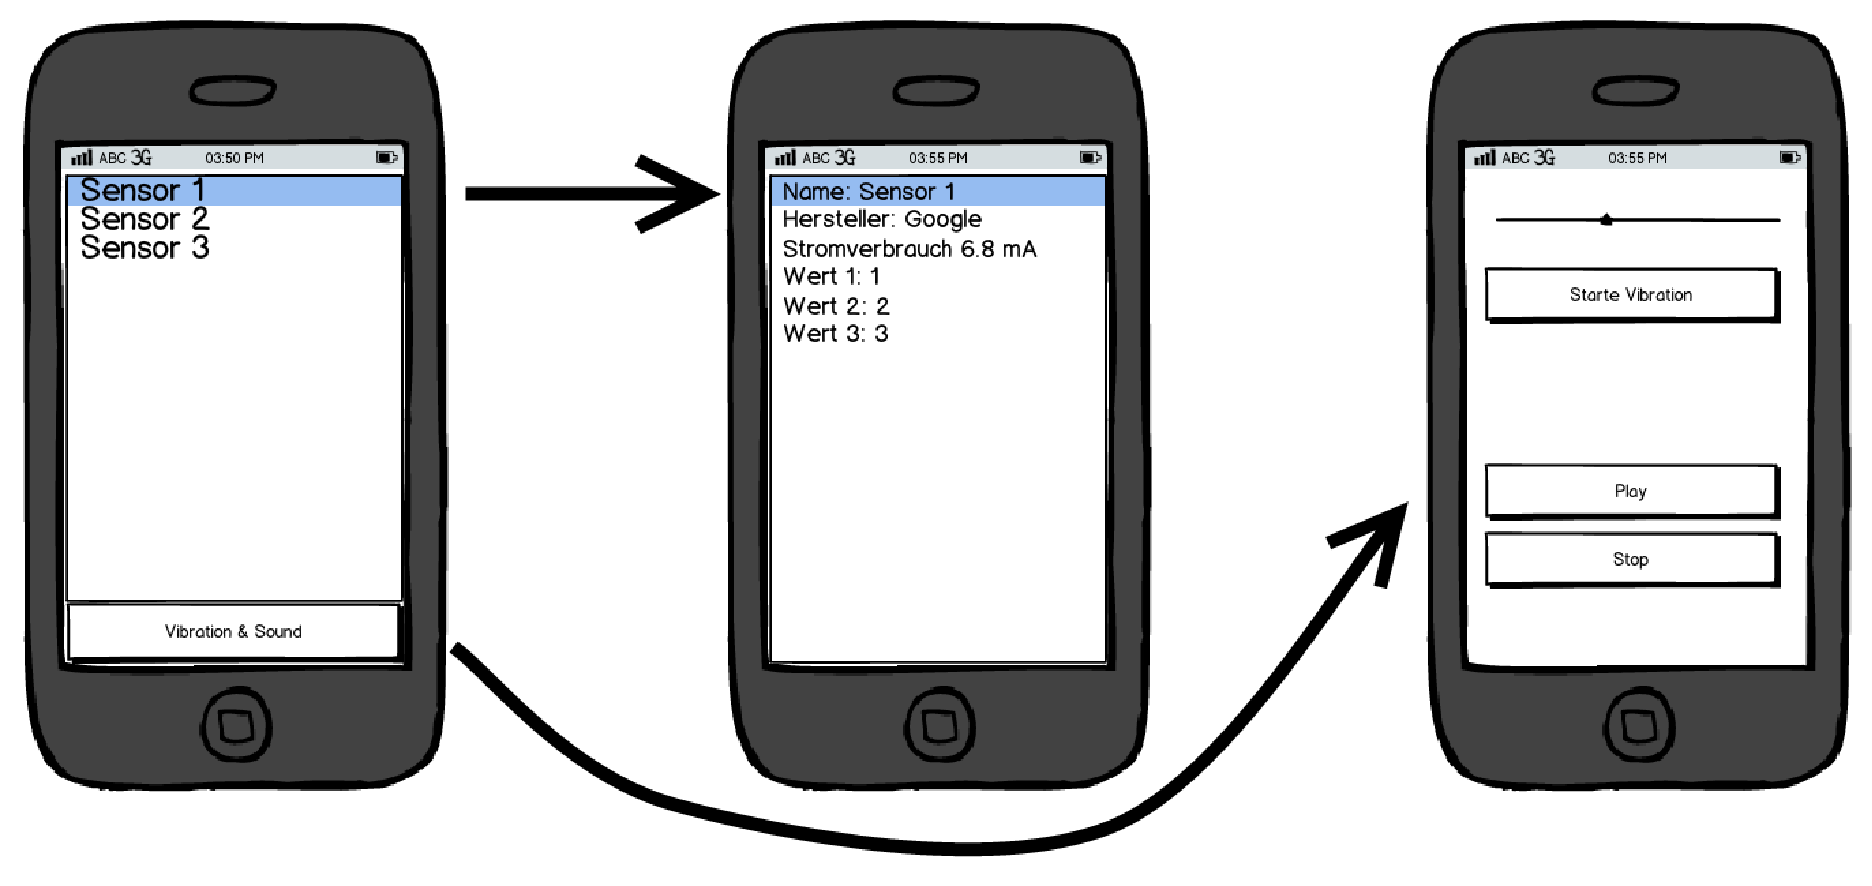
\includegraphics[width=\columnwidth]{example}
    \lfig{example}
    \vspace{-5mm} % use negative white space to fix too large gaps
	\caption{Only include useful figures. Do not simply copy something from a Web.}
\end{figure}

OUR PART:
We propose a modular approach, building first the baseline functionality of the game, followed by further improvements like NAT-punchthrough to allow players from behind different routers to play via the internet with each other or adding more variations and rules. The additional rules will be available to the user of the device the server runs on before game start, such that we can dynamically change the way the game works.\\
Specifically, we would set up a Lookup-server that is reachable for all clients and thus allow the routers to setup forwarding on ports that we know. The LUS can then inform every client about the other client's IP address and ports, through which they can communicate as if they were within the same subnet, as already implemented in the first phase (See ~\rfig{nat}). The gameserver on one phone will have the option to choose whether to use the LUS or only accept players from within the same LAN.\\
\begin{figure}[h]
	\centering
    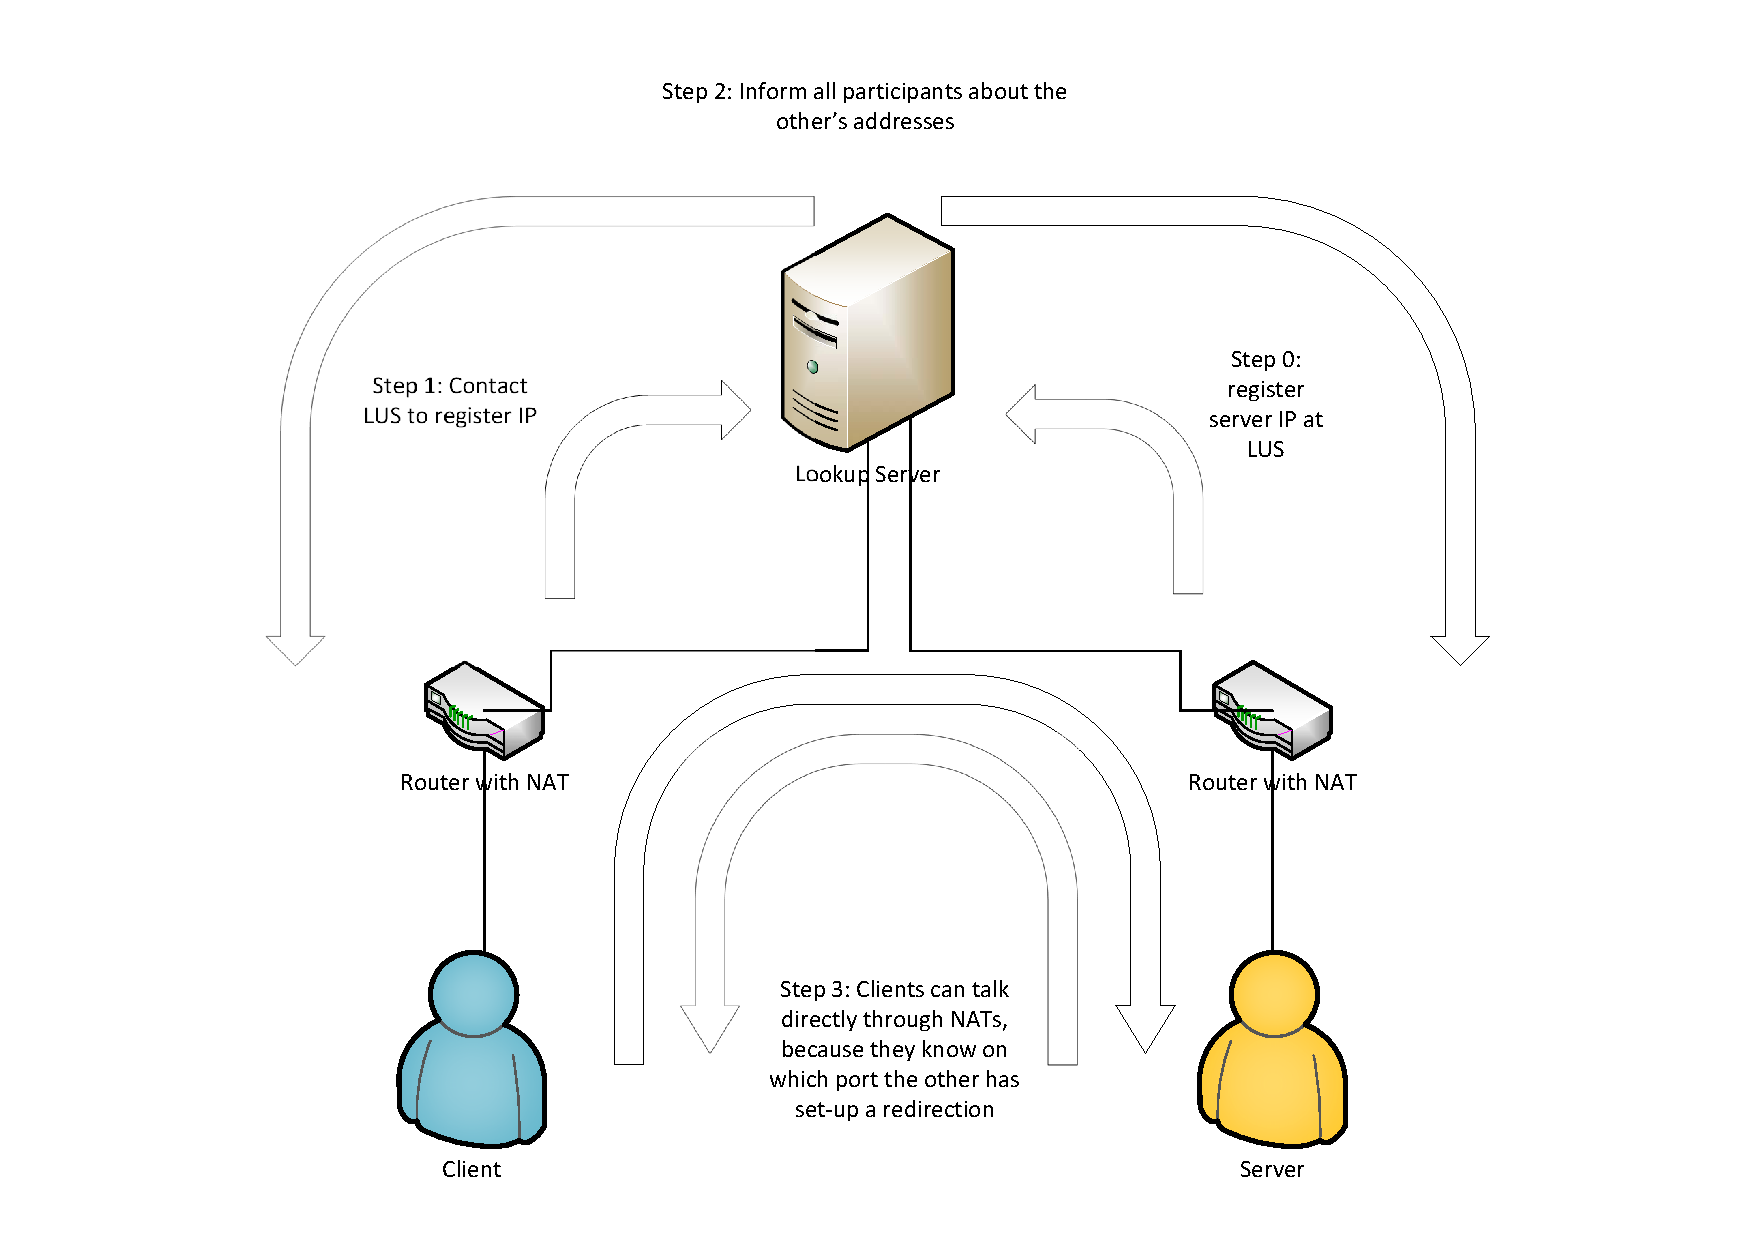
\includegraphics[width=\columnwidth]{NATholepunching.pdf}
    \lfig{nat}
    \vspace{-5mm} % use negative white space to fix too large gaps
	\caption{NAT traversal}
\end{figure}
\\
First of all, we implement a simple server-client setup and define the format and the messages that should be provided as an interface between the client and the server.~\cite{messaging} At the same time, we can start implementing the user interface and writing this proposal.\\
In a second step, once the basic communication between server and client works and the exact behaviour of the two parts has been defined, we implement the serverside game logic and the previously defined messaging functionality.
We will make it so that the server does most of the computations and only sends the client its state, containing the players hand, the number of cards other players are holding and the most recently played cards. The client receives also a list of possible actions, from which it can choose one without having any clientside support for them, except for the user interface. This allows us to later add gamemodes and rules with ease, because we will only need to change a few classes.
We are also trying to keep the classes themselves very modular to make updating them - e.g. by adding further messages - just as simple.\\
Once the game is in a working state with a few rules such as an additional card like the one where the player can choose a color or the well-known "+2" card from UNO, we will decide whether we need to focus on bugfixing, cleaning up code, implementing a LUS or adding more rule options. Adding a LUS might impose additional difficulties because some mobile carriers might use symmetric NATs. If these difficulties arise, we will probably resort to only implementing NAT-traversal for the other (easier) types of NATs.\\
\newline
\newline
TODO: wer macht eine Grafik als überblich zum aufbau und vielleicht noch eine zum UI?


\section{Requirements}
Describe system setup, components, external libraries, hardware etc.


\begin{figure}[h]
	\centering
    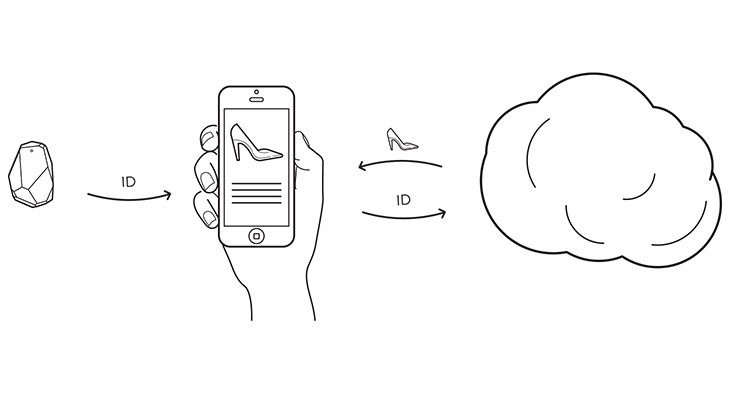
\includegraphics[width=\columnwidth]{overview.jpg}
    \lfig{system-overview}
    \vspace{-5mm} % use negative white space to fix too large gaps
	\caption{System Overview~\cite{estimote}}
\end{figure}

OUR PART:

TODO:Josua beschreibst du das "system setup"?
TODO:jeder der "external libraries, hardware etc." benutz bitte diejenigen beschreiben
\\
Our App runs on Android devices with at least Android 5.0 installed. We use the local wireless connection to communicate between the devices. One device will act as a server and waits for the clients to connect. Once every player is connected the user that started the server can start the game.


\section{Work Packages}
Breakdown the work to subtasks to meet the project requirements.
Define and describe these tasks.

\begin{itemize}
        \item {\bf WP1}:  XYZ  \ldots    
        \item {\bf WP2}: Set and Configuring Backend Serve  \ldots    
        \item {\bf WP3}: Integration  \ldots 
         \item {\bf WPx}:  \ldots 
\end{itemize}
 
Stick to a concise, scientific writing style. 

OUR PART:
There work will be broken down into the following subtasks:
TODO: müsste man den WPs noch andere namen als nummern geben?
TODO: jeder beschreibt das WP für das er verantworlich ist. dürft meine beschreibungen gerne löschen ;)
\begin{itemize}
        \item {\bf WP1}: Define Client-Server Communication\\
        We define the protocol that the client and the server uses to communicate. Once we agreed on a message exchange protocol the developement of the server and the client can be done separately.
        \item {\bf WP2}: Server Game Logic\\
        
           
        \item {\bf WP3}: Client UI
        \item {\bf WP4}: Dynamic Message Parser
        \item {\bf WP5}: Implement Client Server Protocol
\end{itemize}

\section{Milestones}
The milestones section provides a work plan for carrying out the project.
This is your schedule for getting the project done.
Clearly state how the work packages will be distributed among the team members. 

OUR PART:

\subsection{Milestone 1}
\begin{itemize}
	\item Define Client Server Protocol
\end{itemize}

\subsection{Milestone 2}
\begin{itemize}
	\item Getting client server to communicate with the Protocol
\end{itemize}

\subsection{Milestone 3}
\begin{itemize}
	\item Implement Game logic and Client UI
\end{itemize}


We think it is important to have someone who has an overview of the whole project, therefore we assigned a project manager. For the implementation of the application we made two groups, one for the server side and one for the client side. There is one person responsible for the organisation and delegation of the work to other people for both server and client side. These two people also have to set an API to make the two parts work together in the application.

As project manager and organizing the structure of the project: Josua

Server: Responsible for organisation and also helps implementing: Eric, helps with implementation: Fabian

Client: Responsible for organisation and also helps implementing: Chris, helps with implementation: Clemens

UI and Logo: Chris

First responsable for writing the proposal, then helps implementing where there is need: Silvia


% The following two commands are all you need in the
% initial runs of your .tex file to
% produce the bibliography for the citations in your paper.
\bibliographystyle{abbrv}
\bibliography{report}  % sigproc.bib is the name of the Bibliography in this case
% You must have a proper ".bib" file

%\balancecolumns % GM June 2007

\end{document}
